\parindent=1cm %красная строка

\begin{center}
		
		\section{Мультиагентное моделирование системы поддержки принятия решений в составе системы противоракетной обороны}
		
\end{center}

\subsection{Описание системы ПРО} 

Как правило, процесс противоракетной обороны (далее ПРО) состоит из последовательности этапов, включающих ранее обнаружение, отслеживание, распознавание, принятие решения и непосредственный перехват цели, достигаемый посредством взаимодействия всех компонентов системы ПРО (далее СПРО). 

Не вдаваясь в технические подробности и устройство составных компонентов СПРО, отметим только сами компоненты и функции, выполняемые этими компонентами:

\begin{itemize}
	\item Радар раннего обнаружения фиксирует факт запуска ракет и получает приблизительные данные о положении и скорости;
	\item отслеживающий радар <<ведёт>> ракету-перехватчик до завершения перехвата или промаха, получая инструкции из командного центра и передавая их ракете-перехватчику;
	\item командный центр выполняет роль коммуникационного звена и центра обработки информации; производит оценку траектории ракеты, на основании  данных от радара раннего обнаружения; отправляет информацию отслеживающему радару;  создание (генерация) плана перехвата ракеты и отправка его ракете-перехватчику в подходящий момент времени;
	\item ракета-перехватчик выполняет задачу перехвата и способна к ограниченному маневрированию.
\end{itemize} 

Очевидно, что для полного цикла работы СПРО необходима и ракета-цель. 


\subsection{Агентное моделирование и понятие <<агента>>}


Понятие <<агент>> не является строго установленным, но в общем случае можно говорить об <<агенте>> как о сущности, имеющей активность, автономное поведение, способность к самостоятельному приему решений в соответствии  с некоторой заранее заданной совокупностью правил, способность к взаимодействию  с окружающей средой и другими агентами (если такие существуют в рамках модели). Мультиагентные же модели в свою очередь используют множества таких агентов для построения процессов, где поведение системы возникает как следствие взаимодействия множества агентов, а не поведение системы описывает поведение каждого агента, т.е происходит моделирование <<снизу вверх>>.

В рамках данной работы агент будет иметь следующую структуру:
\begin{itemize}
	
	\item сенсор -- получает информацию из внешнего мира в рамках радиуса восприятия;
	\item контроллер -- ядро агента, состоящее из базы априорных знаний, базы правил и системы  принятия решений (СПР)
	\item пр\'{и}вод -- исполняющий компонент агента, ответственный за применение обратной связи к окружающей среде  

\end{itemize}

Примерная структура агента описана схематично на рис. 1.

\begin{figure*}[h!]
	\centering{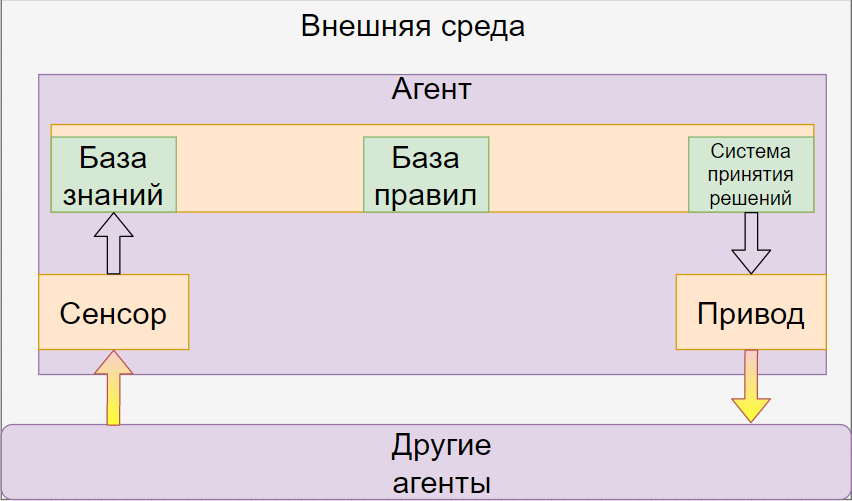
\includegraphics[scale=0.85]{GeneralAgentSchema.png}}
	\caption{Схематическое описание структуры агента и среды}.
\end{figure*} 

Согласно приведенной на рис. 1 схеме, агент способен принимать решения в соответствии с логическими  высказываниями, хранящимися в его базах и / или на основании результатов вычислений. СПР является самой важной частью агента, т.к именно она отвечает за принятие решений. СПР работает по следующему алгоритму: построение модели ограничений на основании данных, полученных из сенсора; выбор наиболее подходящего поведения на основании базы правил и априорной базы знаний.  В целом, СПР может имплементировать механизм дополнительного обучения, позволяющий изменять существующие правила и знания и / или добавлять новые.  

В рамках рассматриваемой в данной работы СПРО, компоненты моделируются с использованием мультиагентного подхода, то есть каждый компонент системы представляет собой агент. СПР решений командного центра СПРО будет генерировать планы перехвата цели динамически, используя для этого данные с радаров обнаружения и вычислительный эксперимент в рамках СПРО. Агенты СПРО показаны на рис. 2. Компоненты одинакового цвета имеют одинаковые возможности. 

\begin{figure*}[h!]
	\centering{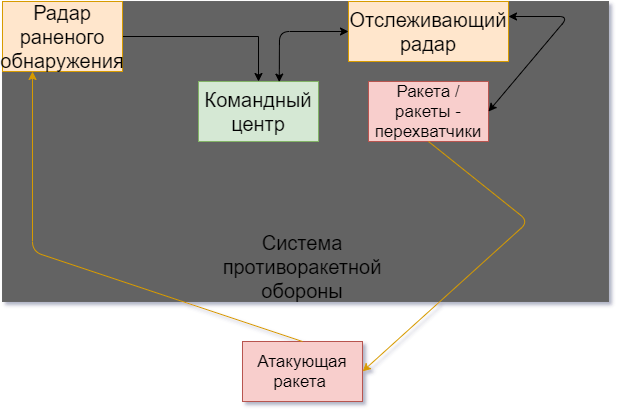
\includegraphics[scale=0.85]{BmdsSchema.png}}
	\caption{Схематическое описание структуры СПРО, связей в ней и воздействия атакующей ракеты}.
\end{figure*} 


\pagebreak


\subsubsection{Агент <<командный центр>>}

Агент <<командный центр>> выполняет назначение конкретной ракеты-перехватчика на цель и посылает инструкции о запуске. Ниже представлена таблица знаний данного агента.

% Please add the following required packages to your document preamble:
% \usepackage{longtable}
% Note: It may be necessary to compile the document several times to get a multi-page table to line up properly
\begin{longtable}{|l|p{0.4\linewidth}|}
	\multicolumn{2}{l}{} \\
	\hline
	Свойство & Значение \\ \hline
	\endfirsthead
	%
	\endhead
	%
	Позиция командного центра (координаты)		& 	широта, долгота, высота	\\ \hline
	Позиция ракеты-перехватчика					&	широта, долгота, высота	\\ \hline 
	Угол наклона ракеты-перехватчика			&	вычисляется с помощью  формул сферической геометрии	     \\ \hline
	Время запуска ракеты-перехватчика			&	вычисляется в рамках решения задачи Ламберта          \\ \hline
	Время подлета ракеты-перехватчика к цели 	&	вычисляется в рамках решения задачи Ламберта         \\ \hline
	Вероятность перехвата						&  	вычисляется ракетой-перехватчиком	     \\ \hline 
	\caption{Таблица знаний командного центра}
	\label{tab:command_center_parameters}\\
\end{longtable}


Правила командного центра включают правила оценки угроз и правила выбора ракеты перехватчика. Эти правила поддерживаются нижеописанной моделью принятия решений.

\textbf{Вычислительная модель назначения ракеты-перехватчика}.
Эта модель генерирует план-назначение ракет-перехватчиков. Для этого используются  местоположение, тип и количество доступных ракет-перехватчиков, уровень угрозы и количество атакующих ракет и время их определения. 

\textbf{Вычислительная модель для точки перехвата}.
Точка перехвата определяется как точка, находящаяся на траектории атакующей ракеты и ближе всего к максимальной высоте ракеты-перехватчика, что позволит запускать дополнительные ракеты в случае неудачи. В свою очередь, траектория атакующей ракеты определяется посредством анализа данных, накапливаемых радаром раннего обнаружения и отслеживающим радаром. Эти данные являются массивом, где каждый элемент имеет вид  <<пара \{координаты, время\} >>.  Максимальная высота, достигаемая ракетой-перехватчиком вычисляется из характеристик этой ракеты, но в данной работе для упрощения вычислений является свойством самой ракеты.

\textbf{Вычислительная модель определения времени запуска ракеты-перехватчика}.
Пусть $T_L$ -- время запуска ракеты-перехватчика; $T_e$ -- момент времени, когда цель окажется в точке перехвата; $T_f$ -- время полета ракеты-перехватчика к точке перехвата; $T_p$ -- время подготовки ракеты-перехватчика к запуску, в данной работе полагаемое константной (однако, можно предположить, что в реальности этот параметр будет вести себя как  модуль квадратичной функции, зависящей от кол-ва подготовленных ракет-перехватчиков, с положительным старшим коэф-том и нулевым дискриминантом, возникающим при приравнивании этой функции нулю). Тогда $T_L = T_e - T_f - T_p$.

\textbf{Модель вычисления угла наклона}
Пусть $A$ -- точка запуска ракеты-перехватчика, $B$ -- предполагаемая точка перехвата, северный полюс --  $C$. Тогда эти три точки вместе с геоцентрической точкой $o$ (центр Земли) формируют сферический треугольный конус; $A, B, C$ представляют угол между двумя гранями, а $a,b,c$  -- геоцентрический угол между двумя точками. Получаем, что угол наклона $\theta_f=arccos(cos(a) \cdot cos(b)+sin(a) \cdot sin(b) \cdot cos(c))$, где 
$a=90-T_{Lat}, b=90-L_{Lat}, C=T_{Lon}-L_{Lon}$, где $L_{Lon}$, $L_{Lat}$ и  $T_{Lon}$, $T_{Lat}$ представляют собой долготу и широту точки запуска и целевой точки перехвата.

\textbf{Модель вычисления параметров уничтожения ракеты-цели}.
Установив начало координат в центр Земли и положив $OX$ как ось, соединяющую центр Земли и точку пуска ракеты, получим полярную систему координат. Обозначим $r_1$, $r_2$, вектор точки запуска и вектор перехвата из геоцентрической точки начала координат; $\theta_f$ -- угол наклона получаемый как $\theta_f = arccos(\frac{r1 \cdot r2}{|r1| \cdot |r2|})$; $\gamma$ -- угол наклона траектории получаемый как $\gamma = \frac{\pi - \theta_f}{4}$ при движении по траектории с минимальной энергией; $\mu$ -- гравитационная константа.    Согласно уравнению Ламберта, скорость перехвата ракеты $V_s$ удовлетворяет условию 
$V_s = \sqrt{\frac{|r_2|(1-cos \theta_f)\mu}{|r_1|^2 \cdot cos(\gamma ^ 2) - |r_2| \cdot  cos(\theta_f + \gamma) \cdot cos \gamma}}$.
Так как траектория полеты -- эллипс, то время полеты ракеты рассчитывается как
$t_f = \frac{|r_1|}{V \cdot cos(\gamma) (\frac{tan(\gamma) (1-cos \theta_f) + (1-\lambda sin \theta_f)}{(2-\lambda)  \frac{|r_1|}{|r_2|}})} + \frac{2cos \gamma}{\lambda ((2/ \lambda) - 1)^{1.5}} arctan \frac{((2-\lambda) - 1) ^ {0.5}}{cos \gamma \cdot ctg(\frac{\theta_f}{2}) - sin \gamma}$, где $\lambda = |r_1| \cdot \frac{V^2}{\mu} $. 


\begin{figure*}[h!]
	\centering{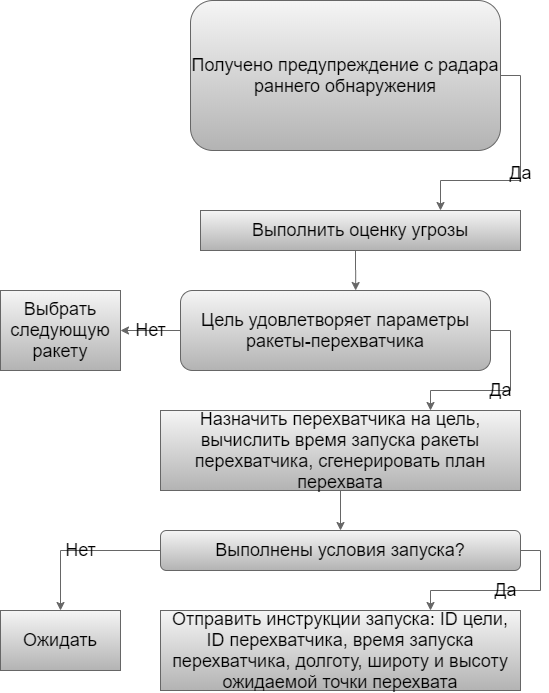
\includegraphics[scale=0.85]{CommandCenterInstruction.png}}
	\caption{Блок схема принятия решения командным центром}.
\end{figure*} 


\subsubsection{Агент <<ракета>>}

В терминах ООП,  <<ракета>> является абстрактным базовым классом, от которого наследуются атакующая ракета и ракета-перехватчик. База его знаний хранит данные, необходимые для вычисления траектории и включает позицию и скорость ракеты, т.е. в каждый момент времени известна широта, долгота, высота и скорость ракеты. 

\begin{figure*}[h!]
	\centering{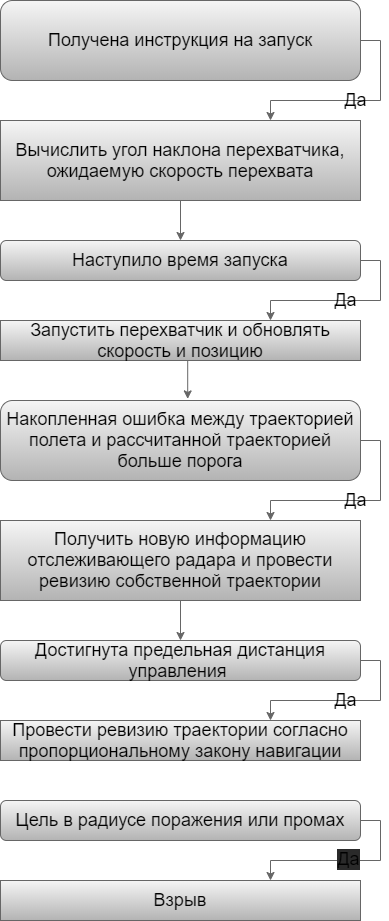
\includegraphics[scale=0.6]{RocketInstruction.png}}
	\caption{Блок схема принятия решения ракетой-перехватчиком}.
\end{figure*} 


\subsubsection{Агент <<радар>>}

Как и в прошлом случае, <<радар>> является абстрактным базовым классом. База знаний радара содержит преимущественно данные для вычисления радиуса радарного покрытия и угла покрытия.   Правила радара включают правила обнаружения и правила предсказания движения ракеты. Правила обнаружения вычисляют область радарного покрытия через радарное уравнение и считается, что любой объект в области радарного покрытия мгновенно обнаруживается при первом сканировании, т.е. в рамках данной работы не рассматриваются цели с активным подавлением радаров или постановкой помех; правила предсказания отсылают информацию в командный центр если объект был замечен хотя бы трижды. 

Полагая, что ракета цилиндрической формы, обозначим $r$ -- радиус ракеты, $h$ -- длина боеголовки, $\lambda$  -- длина волны сигнала радара, $h_1, h_2, h_3$ -- длина двигателей этапа с соответствующим номером. Эффективный поперечник рассеяние (ЭФР) зависит также от угла между радаром и проекций  движения ракеты на  OY, обозначенным как $\theta$ Тогда эффективный поперечник рассеяния ракеты-цели согласно эмпирической формуле равен $R = 2 \pi r (\frac{h_1^2}{\lambda} + \frac{h_2^2}{\lambda} + \frac{h_3^2}{\lambda} + \frac{4}{9 \lambda h} \cdot \sqrt{(r^2+h^2)^3} ) * cos \theta$.

\begin{figure*}[h!]
	\centering{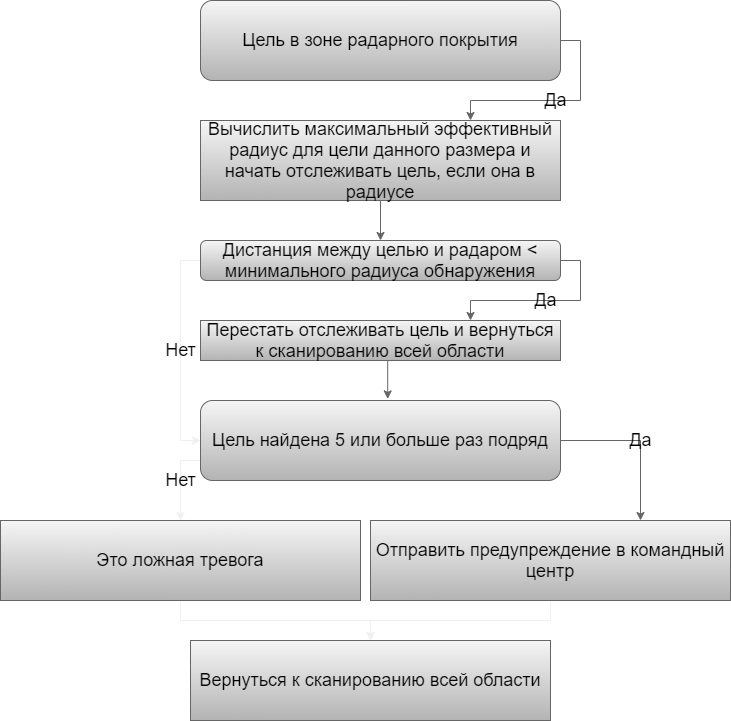
\includegraphics[scale=0.6]{RadarInstruction.png}}
	\caption{Блок схема принятия решения радаром раннего обнаружения}.
\end{figure*} 


\subsection{Система обозначений  и ограничений для алгоритма}

Введем систему обозначений, которые в дальнейшем будут использованы для описания компонентов в алгоритме перехвата целей. 


\begin{longtable}{|l|p{0.4\linewidth}|}
	\multicolumn{2}{l}{} \\
	\hline
	Обозначение & Определение \\ \hline
	\endfirsthead
	%
	\endhead
	%
	n		&	кол-во атакующих ракет-целей	\\ \hline
	j ($\in [0; n]$)		&	номер атакующей ракеты 	\\ \hline
	$T_j$	&	<<угроза>> атакующей ракеты №j	\\ \hline
	$R_j$	&	время на перехват ракеты №j как расстояние от размещения перехватчиков до цели \\ \hline
	$C_j$	&	фактор возможного вмешательства командира	\\ \hline
	$D_j$	&	расстояние от атакующей ракеты №j до цели (цель общая для всех ракет)	\\ \hline
	$S_j$	&	максимальная скорость ракеты №j	\\ \hline
	m		& 	кол-во ракет перехватчиков	\\ \hline
	i ($\in [0; m]$)		&	номер ракеты-перехватчика \\ \hline
	$V_i$	&	<<цена>> ракеты-перехватчика №i	\\ \hline
	$w_k$	&	массив (вектор) специальных весов \\ \hline
	$P_{ij}$ ($P_{ij} \in [0; 1]$)	&	вероятность перехвата ракетой $i$ ракеты $j$	\\ \hline
	$x_{ij}$	&	Булеан, указывающий назначена ли ракета $i$ на ракету $j$	\\ \hline 
	\caption{Символы, используемые для обозначения компонентов алгоритма}
	\label{tab:algorithm_defenitions}\\
\end{longtable}

Отбросим ситуации, где n или m равны 0, т.к. это автоматически приводит к бесконечному множеству решений или пустому множеству решений соответственно. Также заметим, что в рамках этой работы m $\ge$ n.

При решении задачи должны соблюдаться следующие ограничения:

1.Для обеспечения безопасности целей, атакуемых ракетами, необходимо назначить хотя бы одну ракету-перехватчик на каждую цель и приоритет по кол-ву ракет и очередности назначения должен отдаваться ракетам с максимальной <<угрозой>>  и назначаться должны ракеты с минимальной <<стоимостью>>, что позволит избежать быстрого расхода самых <<лучших ракет-перехватчиков>>. Это можно выразить таким фитнесом:
$\sum_{j=1}^{n} \sum_{i=1}^{n}  \frac{T_{j}P_{ij} x_{ij}}{V_{i}x_{ij}}$. 
\newline
2. Генерация плана перехвата зависит от оперативности и качества данных, приходящих с радара. Хорошообнаружимая ракета лучше отслеживается и должна иметь более высокий приоритет.  
\newline
3. Приоритет перехвата также отдается ракетам, более близким к обороняемым целям.
\newline
4. Предпочтительно перехватывать ракеты с более высокой скоростью.
\newline
5. Вмешательство командира, основанное на эмпирическом внешнем знании играет максимальную роль.
\newline
С учетом вышеизложенного, фитнес может быть описан следующим образом 
$\sum_{j=1}^{n}\sum_{i=1}^{m} \frac{P_{ij} \prod_{k=1}^{3}w_k T_j   S_j   C_j}{\prod_{l=4}^{6} w_l V_i x_{ij}  R_j D_j}$.

Для увлечения адаптируемости,  положим $w_x = 1, x \in [1; 6] $ 
\newpage % следующая глава с новой страницы